\begin{frame}[c]{Wolkenfotos}
	\begin{columns}[onlytextwidth]
		\begin{column}{0.2\textwidth}
			\begin{tikzpicture}[scale=1, transform shape]
				\draw circle (1) [path picture={
						\node at (path picture bounding box.center){
						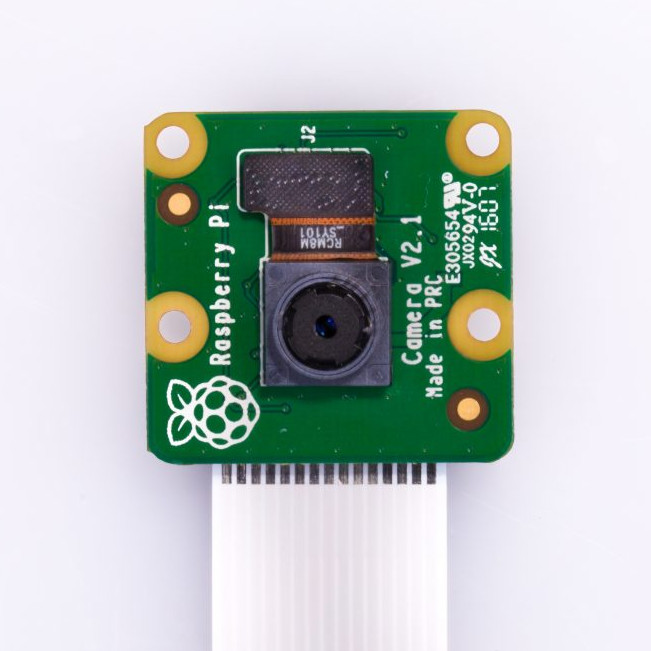
\includegraphics[height=2cm]{picture/picamera.jpg}};},
						line width=1];
				\end{tikzpicture}
			\end{column}
			\begin{column}{0.75\textwidth}
				\begin{block}{PiCamera}
					alle 30 min werden 1024x768 Fotos aufgenommen und die
					Wolkendecke klassifiziert
				\end{block}
			\end{column}
		\end{columns}
		\begin{columns}[onlytextwidth]
			\begin{column}{0.55\textwidth}
				\begin{block}{Motivation}
					Wolkenklassifizierung und -tracking zur Spezifizierung der
					aktuellen Wetterlage und weiterer Parameter f\"ur die
					Vorhersage
				\end{block}
			\end{column}
			\begin{column}{0.4\textwidth}
				\centering
				\begin{tikzpicture}[scale=1, transform shape]
					\draw (0,0) rectangle ++(4,3) [path picture={
							\node at (path picture bounding box.center){
								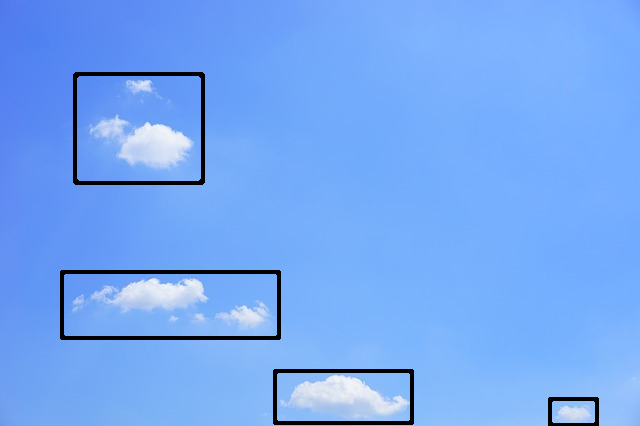
\includegraphics[height=3cm]{picture/cumulus.jpg}};
						}, line width=1] node (F) {};
				\end{tikzpicture}
			\end{column}
		\end{columns}
		\begin{block}{Datenvorbereitung}
			Telegram Bot zum Labeln der Fotos
		\end{block}
	\end{frame}
